\documentclass{article}

\usepackage{graphicx}
\usepackage[spanish]{babel}

\usepackage{listings}
\lstdefinestyle{CStyle}{
	basicstyle=\footnotesize,
	breakatwhitespace=false,
	breaklines=true,
	captionpos=b,
	keepspaces=true,
	numbers=left,
	numbersep=5pt,
	showspaces=false,
	showstringspaces=false,
	showtabs=false,
	tabsize=2,
	language=C
}

\renewcommand{\lstlistingname}{Código}

\title{Programación Orientada al Rendimiento.\\Proyecto de Programación Paralela.}

\author{Grupo 81\\ \\
	Gonzalo Juarez Tello, 100467578\\
	Hodei Urigoitia Merodio, 100374256\\
	Adrián Mancera González, 100429049\\
	Gonzalo Martinez Martín, 100428963
}

\date{}

\begin{document}

\begin{figure}
	
\includegraphics[width=\linewidth,height=0.7\textwidth]{resources/logo_uc3m.png}
\end{figure}
\maketitle
\newpage

\tableofcontents
\newpage

\section{Introducción.\label{intro}}
En esta parte de Programación Orientada al Rendimiento, paralelizamos
el programa simulador de fuerzas ejercidas entre objetos
en un cubo cerrado. Sobre este ejemplo estudiamos el impacto de las
estructuras de datos, los algoritmos, y las optimizaciones secuenciales
y paralelas en el rendimiento\footnote{rendimiento usado como sinónimo de
`tiempo de ejecución'.} final del programa.

Como refresco rápido repasamos primero el diseño secuencial.


En la sección \ref{opt} exploramos las optimizaciones tanto secuenciales como
paralelas que se tuvieron en cuenta. Haciendo comentarios
sobre cuales optimizaciones lograron permanecer en la versión final, cuáles no, y por qué es así.


Luego exponemos los resultados de las pruebas realizadas, los analizamos estadísticamente en la sección \ref{performance},
y cerramos con conclusiones al respecto.

\section{Diseño Original.\label{original}}
En el diseño original de este programa, ambas versiones SoA\footnote{Struct of Arrays} y AoS\footnote{Array of Structs}
son bastante similares. Por lo que consideramos que en este repaso no vale la pena discutir sus diseños por separado.


Una vez superada la inicialización de los objetos. Ambas versiones consitían en 3 loops anidados.
Un loop externo (con variable \textit{k} de manera que $0\leq{k} < {num\_iterations}$)
un loop interno que itera por todos los objetos de uno en uno usando una variable \textit{i}
($0\leq{i} < {num\_objects}$) , y un loop externo que itera por los objetos desde \textit{i}
excluyendo \textit{i} ($i+1\leq{j} < {num\_objects}$).

A lo largo de la memoria, a esta última
parte de los loops anidados con variables \textit{i} y \textit{j} le llamaremos \textbf{doble loop} ó \textbf{loop doble} ().
Su forma básica puede verse en Código \ref{doble_loop:no_striping-no_tiling}.
Es una estructura recurrente en el programa. La variable k desde el vamos no se presta a optimizar porque
necesita la verificación de colisiones antes de cada iteración (tiene una dependencia de datos total
entre una iteración y la otra). El doble loop aparece tanto en chequeo de colisiones, como en cálculo de
fuerzas resultantes de un objeto con el resto.


En cada loop doble se calculan las fuerzas resultantes de un objeto con todos los demás, se aplica la
correspondiente fuerza resultante a cada cuerpo involucrado en el cálculo, y luego se calcula la
aceleración, velocidad, y nueva posición del objeto \textit{i}. La optimización más importante de la
versión original (y la más obvia) es esta de evitar calcular dos veces la fuerza resultante entre
dos objetos. Esto resulta en un espacio de iteración triangular. Que nos es de mucho interés
a la hora de tener en cuenta optimizaciones (sección \ref{opt}). La figura \ref{fig:no_tiling} ilustra
el espacio de iteración del doble loop, así como su flujo de ejecución (indicado por las flechas).


Por último, el diseño original nunca elimina objetos, si no que
los marca. Luego en el código hay condicionales para poder
ignorar aquellos objetos marcados como eliminados.

\begin{lstlisting}[style=CStyle,label=doble_loop:no_striping-no_tiling,caption=doble loop simple.]
for (i = 0; i <= N; ++i)
	for (j = i+1; j <= N; j++)
\end{lstlisting}

\begin{figure}[h!]
	\centering
	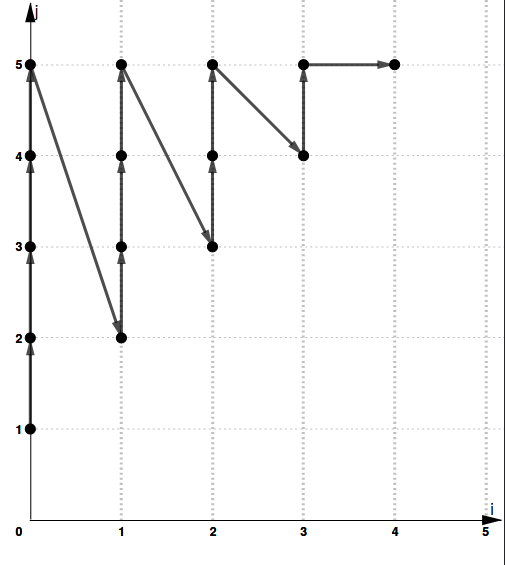
\includegraphics[width=0.6\linewidth,height=0.6\textwidth]{resources/loop_anidado_no_tiling_505x565.png}
	\caption{espacio de iteración de $0\leq{i} < {num\_objects}$, y $i+1\leq{j} < {num\_objects}$
	cuando ${num\_objects}=5$. Las flechas marcan el flujo de ejecución del loop doble.}
	\label{fig:no_tiling}
\end{figure}
%\newpage

\section{Optimizaciones.\label{opt}}

En esta sección discutimos distintas optimizaciones, su impacto en la performance,
y su impacto en los resultados. El tratar con operaciones en punto flotante, el programa
lidia con un trade-off entre precisión en los resultados y mejoras tiempo de ejecución.

\subsection{Optimizaciones secuenciales.\label{opt_seq}}
Las siguientes optimizaciones no solamente intentan mejorar la velocidad
del código de ejecución serializada. Si no también preparar al algoritmo
para poder aprovechar mejor la paralelización a nivel de tarea.

\subsubsection{Vectorización en cálculos de fuerza.\label{simd}}
El título de la subsección \ref{opt_seq} habla de optimizaciones secuenciales, pero para ser honestos,
no es tan así. El paralelismo a nivel de datos puede dar grandes mejoras de rendimiento a aplicaciones
que procesen datos de maneras similares a nuestro programa. Las distintas familias de instrucciones
\textbf{SIMD}\footnote{Single Instruction-Multiple Data} que disponen las arquitecturas x86-64 son
ejemplos de paralelismo a nivel de datos. Estas operaciones son capaces de aplicar la misma operación sobre varios
datos al mismo tiempo.

En nuestro código intentamos sacar ventaja de esto, pero la \textit{vectorización} tiene algunos requisitos.
Evitar dependencias de datos, especialmente de tipo RAW. Y ausencia de estructuras condicionales a no ser
que puedan ser tratadas como \textit{masked assignments}.


El diseño original tiene condicionales dispersos por todo el código. Como se menciona en
la sección \ref{original}, los objetos no se eliminan, se marcan, y su debe verificar su existencia.
Todo esto lo hace la función de chequeo de colisiones. Si esta función se divide en una parte de marcado
de colisiones y fusión de objetos (que no hace más que sumar objeto \textit{a} con objeto \textit{b}), y
una segunda parte donde se eliminen en una sola pasada los objetos marcados y se actualice la longitud
del array de objetos. Entonces el resto del código no necesita condicionales para verificar la existencia de objetos.


Otra restricción para que el compilador pueda vectorizar el código, es la \textit{supresión de dependencias de datos}.
En particular y como mínimo, evitar \textit{RAW} (al menos en x86-64). El cálculo de fuerzas tiene de esto en algunas
partes. Por ejemplo, el objeto en el índice del loop menos profundo \textit{i}, tiene dependencias WAW entre iteraciones.
O bien, hay dependencias RAW propias de utilizar el resultado de un cálculo almacenado en una variable, para un nuevo cálculo.


Una técnica llamada \textit{strip-mining} presentada en \ref{strip-mining} permite exponer la vectorización
del algoritmo, así como eliminar algunas dependencias WAW (convertir variables únicas en arrays). No es
la única utilidad que se le da en el código pero en esta sección es lo que nos importa.


Para lidiar con RAW, una posible solución es la de dividir un loop con RAW en 2 loops sin RAW (también
facilitado por strip-mining. Pero esto puede resultar en una pérdida de rendimiento, por lo tanto
hay que medir.


Como nota: la función para obtener raíz cuadradas no es vectorizable a no ser que se utilice una flag
del compilador que permite su aproximación por métodos numéricos. Esta estimación está bien hasta
cierto número de iteraciones y objetos donde el error que arrastra se vuelve imperdonable.


El código original no pareció incorporar muy bien las instrucciones SIMD en el cálculo de fuerzas.
Por alguna razón, incluso eliminando las dependencias de datos, el compilador se rehúsa a vectorizar
una parte caliente\footnote{parte del programa accedida con mucha frecuencia} del código, y obligarlo
con la directiva \textit{\#pragma omp simd} no termina en buenos resultados ni performance.

\subsubsection{Strip-Mining.\label{strip-mining}}
Strip-mining es una técnica que permite exponer oportunidades de vectorización al compilador, como es mencionado
en la subsección \ref{simd}. Varias veces el compilador puede llevar a cabo esta optimización por su cuenta.


También permite mejorar la localidad tanto espacial como temporal si los mismos datos son utilizados en distintas partes
del algoritmo. Este último uso es el que se le dá en la versión final del código para el cálculo de fuerzas.


Si N es el tamaño del array a recorrer, se utiliza un tamaño de \textit{stride} ó \textit{step} para que una variable \textit{ii}
tome valores $0\leq{ii}\leq N$ avanzando cada iteración el valor del step. Luego la variable \textit{i} original puede recorrer
el tamaño de \textit{stride} de uno en uno. Esto aplicado a \textit{loop doble}, lo deja expresado de como se lo ve en
Código \ref{doble_loop:striping-no_tiling}.

Es importante aclarar que strip-mining por sí solo no altera el orden de ejecución del programa. Por lo
que el gráfico de Figura \ref{fig:no_tiling} sigue aplicando.

\begin{lstlisting}[style=CStyle,label=doble_loop:striping-no_tiling,caption=doble loop con strip-mining en ambos loops.]
/* strip-mining de cabecera de loop 1 */
for (ii = 0; ii <= N; ii+=stride)
for (i = ii; i <= min(ii+stride-1, N); ++i)
	/* strip-mining de cabecera de loop 2 */
	for (jj = i+1; jj <= N; jj+=stride)
	for (j = jj; j <= min(jj+stride-1, N); j++)
\end{lstlisting}


El código final también hace uso de la técnica para evitar false-sharing, algo que se explica con mas profundidad
en \ref{strip-mining-parallel}, la sección de esta técnica en las optimizaciones paralelas.

\subsubsection{Loop-tiling en loops anidados.}

Loop-tiling es una técnica para mejorar la localidad temporal en loops anidados de n-dimensiones\footnote{profundidad del anidado de loops}.
Básicamente consiste en 2 pasos: strip-mining, y permutación loops.

El procedimiento de strip-mining es el explicado en la subsección \ref{strip-mining}.
\begin{equation}
	\begin{array}{rrr}
		\left\{
			\begin{array}{r}
			1+2\leq3\\
			3+4\geq7
			\end{array}
		\right.
		&
		\textit{se convierte en}
		&
		\left\{
			\begin{array}{r}
			1+2\leq3\\
			3+4\geq7
			\end{array}
		\right.
	\end{array}
\end{equation}
\subsubsection{Flags de compilador.}

\subsection{Optimizaciones con paralelismo.\label{opt_parallel}}

\subsubsection{Paralelización en cálculos de fuerza.}

\subsubsection{Uso de Strip-Mining para paralelismo.\label{strip-mining-parallel}}

\subsection{Conclusiones sobre las optimizaciones.}

\section{Diseño Final.\label{final}}
\subsection{AOS paralelo.}
\subsection{SOA paralelo.}

\section{Evaluación de Rendimiento.\label{performance}}
\subsection{Resultados obtenidos.}
\subsection{Secuencial vs. Paralelo.}
\subsection{Interpretación de resultados y pruebas.}

\section{Conclusiones Finales.\label{conclusiones}}

\end{document}
